%% abtex2-modelo-trabalho-academico.tex, v-1.7.1 laurocesar
%% Copyright 2012-2013 by abnTeX2 group at http://abntex2.googlecode.com/ 
%%
%% This work may be distributed and/or modified under the
%% conditions of the LaTeX Project Public License, either version 1.3
%% of this license or (at your option) any later version.
%% The latest version of this license is in
%%   http://www.latex-project.org/lppl.txt
%% and version 1.3 or later is part of all distributions of LaTeX
%% version 2005/12\usepackage{array}/01 or later.
%%
%% This work has the LPPL maintenance status `maintained'.
%% 
%% The Current Maintainer of this work is the abnTeX2 team, led
%% by Lauro César Araujo. Further information are available on 
%% http://abntex2.googlecode.com/
%%
%% This work consists of the files abntex2-modelo-trabalho-academico.tex,
%% abntex2-modelo-include-comandos and abntex2-modelo-references.bib
%%

% ------------------------------------------------------------------------
% ------------------------------------------------------------------------
% abnTeX2: Modelo de Trabalho Academico (tese de doutorado, dissertacao de
% mestrado e trabalhos monograficos em geral) em conformidade com 
% ABNT NBR 14724:2011: Informacao e documentacao - Trabalhos academicos -
% Apresentacao
% ------------------------------------------------------------------------
% ------------------------------------------------------------------------

\documentclass[
	% -- opções da classe memoir --
	12pt,				% tamanho da fonte
	openright,			% capítulos começam em pág ímpar (insere página vazia caso preciso)
	oneside,			% para impressão em verso e anverso. Oposto a oneside
	a4paper,			% tamanho do papel. 
	% -- opções da classe abntex2 --
	%chapter=TITLE,		% títulos de capítulos convertidos em letras maiúsculas
	%section=TITLE,		% títulos de seções convertidos em letras maiúsculas
	%subsection=TITLE,	% títulos de subseções convertidos em letras maiúsculas
	%subsubsection=TITLE,% títulos de subsubseções convertidos em letras maiúsculas
	% -- opções do pacote babel --
	english,			% idioma adicional para hifenização
	french,				% idioma adicional para hifenização
	spanish,			% idioma adicional para hifenização
	brazil,				% o último idioma é o principal do documento
	]{ufsj-abntex2}


% ---
% PACOTES
% ---

% ---
% Pacotes fundamentais 
% ---
\usepackage{cmap}				% Mapear caracteres especiais no PDF
\usepackage{lmodern}			% Usa a fonte Latin Modern			
\usepackage[T1]{fontenc}		% Selecao de codigos de fonte.
\usepackage[utf8]{inputenc}		% Codificacao do documento (conversão automática dos acentos)
\usepackage{lastpage}			% Usado pela Ficha catalográfica
\usepackage{indentfirst}		% Indenta o primeiro parágrafo de cada seção.
\usepackage{color}				% Controle das cores
\usepackage[pdftex]{graphicx}
\usepackage{array}
\usepackage{verbatim}
\usepackage{multirow}
\usepackage{footnote}
\usepackage{subfigure}
\usepackage{nameref}
\usepackage{footmisc}
\usepackage{float}
\usepackage{longtable}
\usepackage{caption}

\setlength\extrarowheight{2pt}
% ---
		
% ---
% Pacotes adicionais, usados apenas no âmbito do Modelo Canônico do abnteX2
% Provê somente o comando \lipsum, para gerar texto aleatório.
% Já que estes comandos serão retirados, pode ser excluída também.
% ---
\usepackage{lipsum}				% para geração de dummy text
% ---
% ---
% Pacotes de citações
% ---
\usepackage[brazilian,hyperpageref]{backref}	 % Paginas com as citações na bibl
\usepackage[alf]{abntex2cite}	% Citações padrão ABNT

% --- 
% CONFIGURAÇÕES DE PACOTES
% --- 

% ---
% Configurações do pacote backref
% Usado sem a opção hyperpageref de backref
\renewcommand{\backrefpagesname}{Citado na(s) página(s):~}
% Texto padrão antes do número das páginas
\renewcommand{\backref}{}
% Define os textos da citação
\renewcommand*{\backrefalt}[4]{
	\ifcase #1 %

	\or
		Citado na página #2.%
	\else
		Citado #1 vezes nas páginas #2.%
	\fi}%
% ---


% ---
% Informações de dados para CAPA e FOLHA DE ROSTO
% ---
%\titulo{Heurísticas aplicadas ao problema de projeto de redes de telecomunicações com qualidade de serviço}
\titulo{Netflix Movies \& TV Shows: Estudo, análise e descoberta de conhecimento na rede}
\autor{Antônio Marcos Machado Bernardes\\Ronan José Lopes}
\local{Universidade Federal de São João del-Rei}
\data{2021}
% \orientador{Elisa de Tuler Albergaria}
% \coorientador{Co-orientador} % se não existir, comente essa linha



% ---
% Configurações de aparência do PDF final

% alterando o aspecto da cor azul
%\definecolor{blue}{RGB}{41,5,195}
\definecolor{blue}{RGB}{0,0,0}

% informações do PDF
\makeatletter
\hypersetup{
     	%pagebackref=true,
		pdftitle={\@title}, 
		pdfauthor={\@author},
    	pdfsubject={\imprimirpreambulo},
	    pdfcreator={LaTeX with abnTeX2},
		pdfkeywords={abnt}{latex}{abntex}{abntex2}{trabalho acadêmico}, 
		colorlinks=true,       		% false: boxed links; true: colored links
    	linkcolor=blue,          	% color of internal links
    	citecolor=blue,        		% color of links to bibliography
    	filecolor=magenta,      		% color of file links
		urlcolor=blue,
		bookmarksdepth=4
}
\makeatother

% --- 

% --- 
% Espaçamentos entre linhas e parágrafos 
% --- 

% O tamanho do parágrafo é dado por:
\setlength{\parindent}{1.3cm}

% Controle do espaçamento entre um parágrafo e outro:
\setlength{\parskip}{0.2cm}  % tente também \onelineskip

% ---
% compila o indice
% ---
\makeindex
% ---

\pagestyle{headings}
\setcounter{page}{1}
\pagenumbering{arabic}

% ----
% Início do documento
% ----
\begin{document}

% Retira espaço extra obsoleto entre as frases.
\frenchspacing 

% ----------------------------------------------------------
% ELEMENTOS PRÉ-TEXTUAIS
% ----------------------------------------------------------
 \pretextual

% ---
% Capa
% ---
\imprimircapa
% ---


% ---
% Inserir a ficha bibliografica
% ---
%% Isto é um exemplo de Ficha Catalográfica, ou ``Dados internacionais de
% catalogação-na-publicação''. Você pode utilizar este modelo como referência. 
% Porém, provavelmente a biblioteca da sua universidade lhe fornecerá um PDF
% com a ficha catalográfica definitiva após a defesa do trabalho. Quando estiver
% com o documento, salve-o como PDF no diretório do seu projeto e substitua todo
% o conteúdo de implementação deste arquivo pelo comando abaixo:
%
% \begin{fichacatalografica}
%     \includepdf{fig_ficha_catalografica.pdf}
% \end{fichacatalografica}
\begin{fichacatalografica}
	\vspace*{\fill}					% Posição vertical
	\hrule							% Linha horizontal
	\begin{center}					% Minipage Centralizado
	\begin{minipage}[c]{12.5cm}		% Largura
	
	\imprimirautor
	
	\hspace{0.5cm} \imprimirtitulo  / \imprimirautor. --
	\imprimirlocal, \imprimirdata-
	
	\hspace{0.5cm} \pageref{LastPage} p. : il. (algumas color.) ; 30 cm.\\
	
	\hspace{0.5cm} \imprimirorientadorRotulo~\imprimirorientador\\
	
	\hspace{0.5cm}
	\parbox[t]{\textwidth}{\imprimirtipotrabalho~--~\imprimirinstituicao,
	\imprimirdata.}\\
	
	\hspace{0.5cm}
		1. Palavra-chave1.
		2. Palavra-chave2.
		I. Orientador.
		II. Universidade Federal de São João del-Rei.
		III. Ciência da Computação.
		IV. Título\\ 			
	
	\hspace{8.75cm} CDU 02:141:005.7\\
	
	\end{minipage}
	\end{center}
	\hrule
\end{fichacatalografica}
% ---

% ---
% Inserir errata - Elemento opcional. Caso não utilize, basta comentar a linha
% ---
%\begin{errata}
Elemento opcional da \citeonline[4.2.1.2]{NBR14724:2011}. Exemplo:

\vspace{\onelineskip}

FERRIGNO, C. R. A. \textbf{Tratamento de neoplasias ósseas apendiculares com
reimplantação de enxerto ósseo autólogo autoclavado associado ao plasma
rico em plaquetas}: estudo crítico na cirurgia de preservação de membro em
cães. 2011. 128 f. Tese (Livre-Docência) - Faculdade de Medicina Veterinária e
Zootecnia, Universidade de São Paulo, São Paulo, 2011.

\begin{table}[htb]
\center
\footnotesize
\begin{tabular}{|p{1.4cm}|p{1cm}|p{3cm}|p{3cm}|}
  \hline
   \textbf{Folha} & \textbf{Linha}  & \textbf{Onde se lê}  & \textbf{Leia-se}  \\
    \hline
    1 & 10 & auto-conclavo & autoconclavo\\
   \hline
\end{tabular}
\end{table}

\end{errata}
% ---

% ---
% Inserir folha de aprovação
% ---
%% Isto é um exemplo de Folha de aprovação, elemento obrigatório da NBR
% 14724/2011 (seção 4.2.1.3). Você pode utilizar este modelo até a aprovação
% do trabalho. Após isso, substitua todo o conteúdo deste arquivo por uma
% imagem da página assinada pela banca com o comando abaixo:
%
% \includepdf{folhadeaprovacao_final.pdf}
%
\begin{folhadeaprovacao}

  \begin{center}
    {\ABNTEXchapterfont\large\imprimirautor}

    \vspace*{\fill}\vspace*{\fill}
    {\ABNTEXchapterfont\bfseries\Large\imprimirtitulo}
    \vspace*{\fill}
    
    \hspace{.45\textwidth}
    \begin{minipage}{.5\textwidth}
        \imprimirpreambulo
    \end{minipage}%
    \vspace*{\fill}
   \end{center}
    
   Trabalho aprovado. \imprimirlocal, 17 de janeiro de 2014:

   \assinatura{\textbf{\imprimirorientador} \\ Orientador} 
   \assinatura{\textbf{Carolina Ribeiro Xavier} \\ Convidado 1}
   \assinatura{\textbf{Daniel Ludovico Guidoni} \\ Convidado 2}
   %\assinatura{\textbf{Professor} \\ Convidado 3}
   %\assinatura{\textbf{Professor} \\ Convidado 4}
      
   \begin{center}
    \vspace*{0.5cm}
    {\large\imprimirlocal}
    \par
    {\large\imprimirdata}
    \vspace*{1cm}
  \end{center}
  
\end{folhadeaprovacao}

% ---

% ---
% Dedicatória, Agradecimento e Epígrafe
% ---
%% ---
% Dedicatória
% ---
\begin{dedicatoria}
   \vspace*{\fill}
   \centering
   \noindent
   \textit{ Este trabalho é dedicado às crianças adultas que,\\
   quando pequenas, sonharam em se tornar cientistas.} \vspace*{\fill}
\end{dedicatoria}

% ---
% Agradecimentos
% ---
\begin{agradecimentos}
Os agradecimentos principais são direcionados à Gerald Weber, Miguel Frasson,
Leslie H. Watter, Bruno Parente Lima, Flávio de Vasconcellos Corrêa, Otavio Real
Salvador, Renato Machnievscz\footnote{Os nomes dos integrantes do primeiro
projeto abn\TeX\ foram extraídos de
\url{http://codigolivre.org.br/projects/abntex/}} e todos aqueles que
contribuíram para que a produção de trabalhos acadêmicos conforme
as normas ABNT com \LaTeX\ fosse possível.

Agradecimentos especiais são direcionados ao Centro de Pesquisa em Arquitetura
da Informação\footnote{\url{http://www.cpai.unb.br/}} da Universidade de
Brasília (CPAI), ao grupo de usuários
\emph{latex-br}\footnote{\url{http://groups.google.com/group/latex-br}} e aos
novos voluntários do grupo
\emph{\abnTeX}\footnote{\url{http://groups.google.com/group/abntex2} e
\url{http://abntex2.googlecode.com/}}~que contribuíram e que ainda
contribuirão para a evolução do \abnTeX.

\end{agradecimentos}
% ---

% ---
% Epígrafe
% ---
\begin{epigrafe}
    \vspace*{\fill}
	\begin{flushright}
		\textit{``Não vos amoldeis às estruturas deste mundo, \\
		mas transformai-vos pela renovação da mente, \\
		a fim de distinguir qual é a vontade de Deus: \\
		o que é bom, o que Lhe é agradável, o que é perfeito.\\
		(Bíblia Sagrada, Romanos 12, 2)}
	\end{flushright}
\end{epigrafe}
% ---
% ---


% ---
% inserir o sumario
% ---
\pdfbookmark[0]{\contentsname}{toc}
\tableofcontents*
% ---



% ----------------------------------------------------------
% ELEMENTOS TEXTUAIS
% ----------------------------------------------------------
%\textual

% ----------------------------------------------------------
% Introdução
% ----------------------------------------------------------
\chapter[Introdução]{Introdução}

No contexto da ciência da computação, a área de estudo de redes complexas fornece uma abstração para estudo de sistemas onde os elementos desse sistema realizam algum tipo de interação entre si. Essa abstração toma como base o modelo e estrutura de dados dos grafos e possibilita, através da análise de propriedades estruturais e métricas que fornecem indicadores do comportamento da rede, descrever e compreender melhor o sistema como um todo. Como uma área de aplicação multidisciplinar, pode ser utilizada em aplicações biológicas, análise de tráfego de veículos, interações em redes sociais, dentre outros vários exemplos possíveis.

A fim demonstrar um possível caso de uso, o estudo a ser aqui desenvolvido toma como objeto de estudo a base "Netflix Movies and TV Shows"\footnote{\href{https://www.kaggle.com/shivamb/netflix-shows}{https://www.kaggle.com/shivamb/netflix-shows}}, que contém informações relevantes sobre filmes e séries disponíveis no serviço de \textit{streaming} e foi disponibilizada na rede de descoberta de conhecimento Kaggle. Dentre as sugestões de estudo e análise sugeridas na publicação da base, o tópico "Análise de rede de atores/diretores para encontrar insights interessantes" é um exemplo direto de aplicação de estudo da disciplina de redes complexas.

Nas seções seguintes, são detalhadas as propostas de análise e hipóteses a serem testadas na rede mencionada. O estudo desenvolvido tem como ponto de partida uma compreensão rasa acerca da rede tal como descrito no parágrafo anterior e, progressivamente, clarifica melhor o processo de geração, comportamento e predições relativos ao sistema em análise.

% ----------------------------------------------------------
% Parte de revisãod e literatura
% ----------------------------------------------------------
%\part{Revisão de Literatura}

\chapter{Detalhamento do Problema Proposto}
A proposta do trabalho aqui desenvolvido consiste em implementar os algoritmos em foco (InsertionSort, MergeSorte e, a partir da utilização das funções implementadas nestes, o algoritmo híbrido TimSort). Para testar o funcionamento das rotinas implementadas, algumas entradas a serem processadas devem ser geradas. A fim de explorar diferentes conjunturas, de forma que um algoritmo em particular não se beneficie do formato do conjunto a ser ordenado, os seguintes cenários são determinados para geração das entradas:

\begin{itemize}
	\item Vetor gerado com elementos em posição completamente aleatória
	\item Vetor gerado com elementos em ordem crescente
	\item Vetor gerado com elementos em ordem decrescente
\end{itemize}

Para avaliar também como os algoritmos se comportam à medida que o tamanho da entrada cresce, os vetores gerados possuem tamanhos 32, 64, 1.024, 10.000, 100.000 e 1.000.000. Esse desempenho será medido em termos de tempo de processamento efetivo e também em número de operações relevantes dentro do algoritmo (como trocas de posição e comparação de maior/menor). Como a medida do tempo em um sistema operacional oscila devido à concorrência dos processos pela CPU, para cada um desses contextos serão feitas 10 execuções, com o intuito de se obter uma média mais confiável. Isso gera um total de 180 execuções (3 configurações de entrada x 6 tamanhos de entrada x 10 execuções) para cada algoritmo. 

A partir dos resultados obtidos, será verificado o comportamento assintótico na prática condiz com a análise de complexidade teórica destes algoritmos. Esta tem por finalidade descrever o comportamento de determinada rotina à medida que o tamanho da entrada a ser processada cresce. Além disso, fornece uma análise dos casos de pior, melhor e médio desempenho de cada algoritmo, de forma a auxiliar a escolha de acordo com a característica dos conjuntos de dados que serão efetivamente ordenados na aplicação.


% Aqui entram os capitulos contendo a revisão de literatura
% ---
% Capitulo de revisão de literatura
% ---

\chapter{Análise da Rede}

\section{Sumarização de indicadores descritivos}

De imediato, é possível aferir alguns dados básicos da rede completa com o auxílio do \textit{Networkx} ou do \textit{Gephi}:

\begin{itemize}
	\item Número de nós: 32.881 (maior do que o número de registros pois cada registro contém um elenco com N atores/atrizes)
	\item Número de arestas: 252.055
	\item Grau médio:  15,33 (média de ligações/interações de cada vértice/ator)
\end{itemize}

Conforme descrito na modelagem da rede, optou-se pro obter o sub-grafo da componente gigante da rede, cuja cobertura inclui cerca de 89,5\% dos vértices da rede:

\begin{itemize}
	\item Número de vértices: 29.440
	\item Número de arestas: 241.744
	\item Grau médio:  16,42
	\item Densidade: 0,000557 (Razão entre número de arestas existentes/possíveis)
	\item Diâmetro: 17 (caminho mais longo possível entre quaisquer 2 vértices da rede)
	\item Coeficiente de \textit{clustering} médio: 0,824 (Alta probabilidade devido às “aglomerações locais” do \textit{elenco} de cada registro, onde todos os nós têm ligações entre si)
	\item Comprimento médio de caminho: 5,647 (Distância média, em númeo de vértices, que deveria ser percorrida para alcance entre dois vértices arbitrários)
	\item Fechamento triadíco: 0,39849 (Probabilidade de formação de “triângulos” - relativamente alta pelo mesmo motivo do coeficiente de \textit{clustering})

\end{itemize}

A figura \ref{fig:grau-netflix} auxilia na visualização de como os graus dos vértices da rede estão distribuídos. A distribuição é exibida de forma que o eixo X representa a cardinalidade possível do grau do vértice de acordo com as ocorrências na base, enquanto no eixo Y está representado sua probabilidade, de acordo com o número efetivo de ocorrências. O grau 9 (ou seja, o ator/atriz co-atuar com 9 outros atores), por exemplo, de maior ocorrência, tem uma probabilidade um pouco maior que 16\%.

\begin{figure}[!htb]
\centering
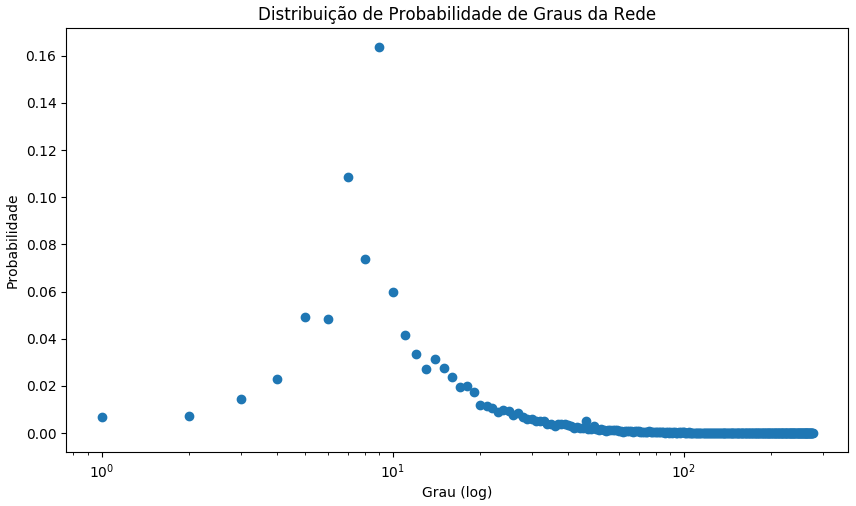
\includegraphics[width=13cm]{img/grau-probabilidade-netflix.png}
\caption{Distribuição de graus da rede x probabilidade de ocorrência}
\label{fig:grau-netflix}
\end{figure}


\section{Detecção de comunidades}

Para detecção de comunidades na rede, foram utilizados os algoritmos de modularidade e método de Louvain (que consiste em um aprimoramento do método anterior) respectivamente no Networkx e no Gephi. Pelo método de Louvain, foram obtidas 93 comunidades, contendo a maior delas 4.823 vértices, a menor 5 vértices, e uma média de 313,19 vértices por comunidade. No Gephi, o método de modularidade gerou 99 comunidades.

\begin{figure}[!htb]
\centering
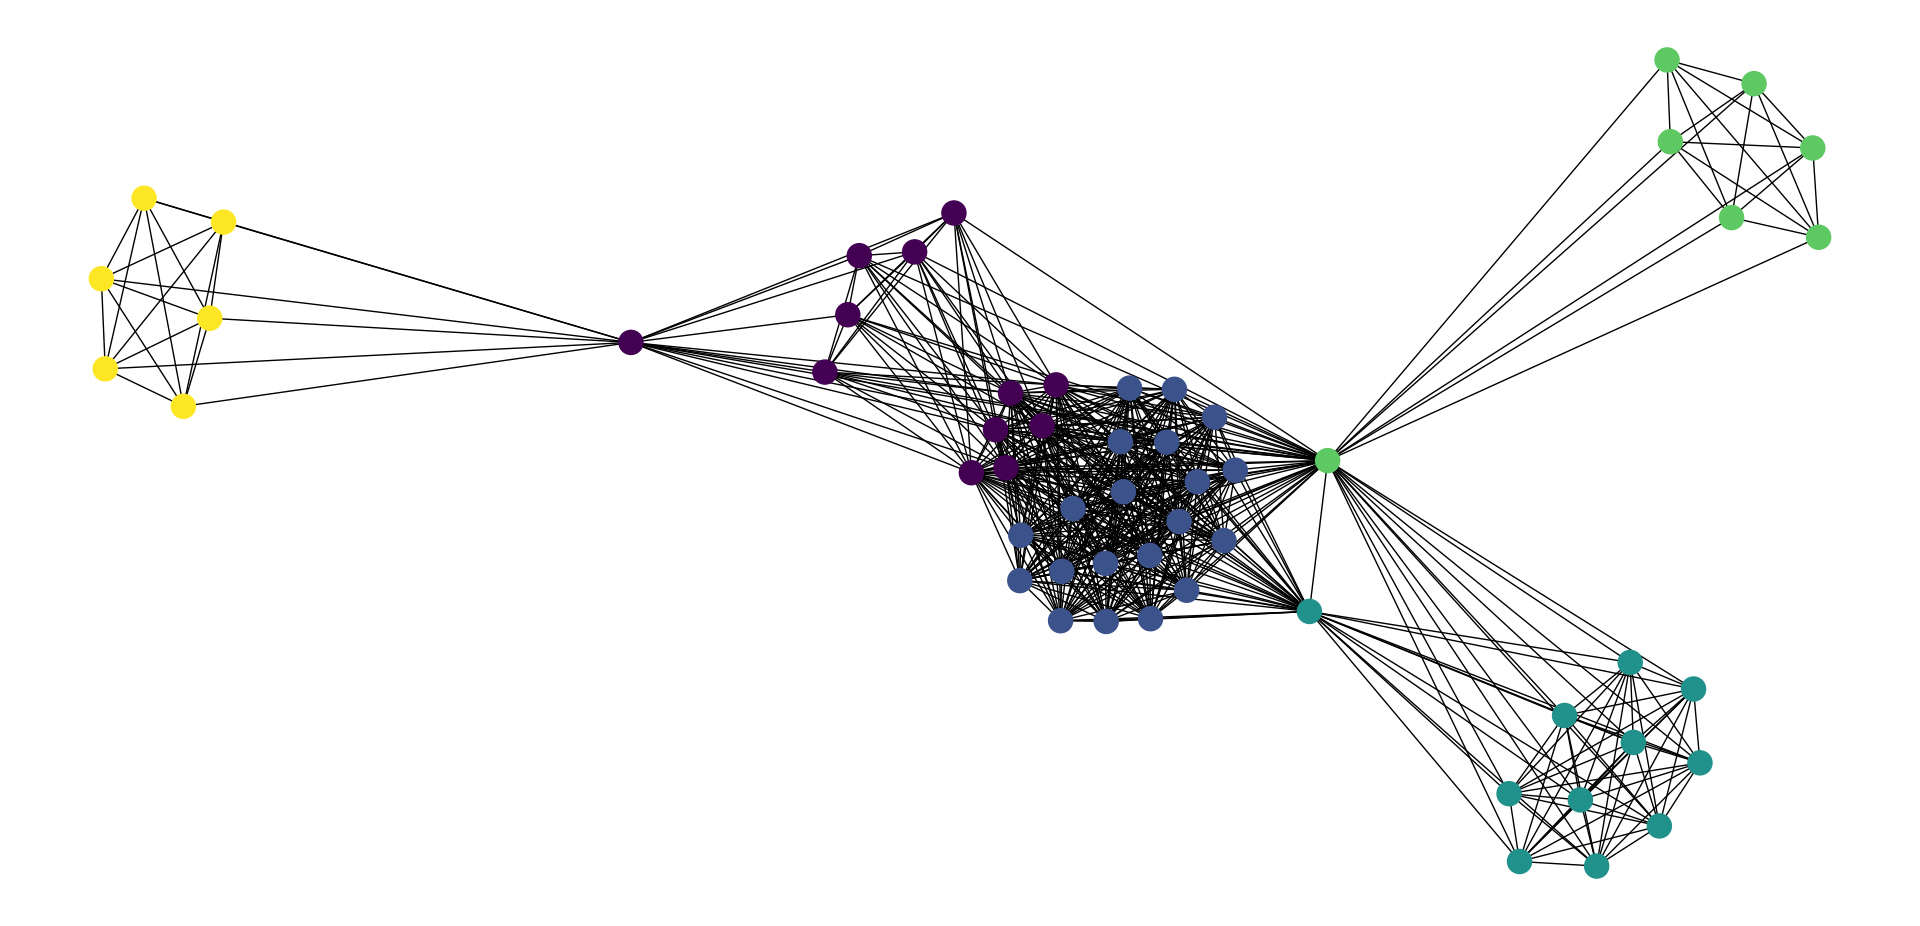
\includegraphics[width=14cm]{img/Figure_3.png}
\caption{Divisão de comunidades no NetworkX - Método de Louvain}
\label{fig:sub-comunidades}
\end{figure}

A figura \ref{fig:sub-comunidades} ilustra, para uma amostra pequena, uma ideia da divisão de comunidades no NetworkX. Pela característic ada modelagem da rede, espera-se esse comportamento onde hajam vários pequenos grupos conectados (correspondentes aos elencos individualmente) e alguns vértices como é possível observar na imagem que fazem essas pontes dentre os aglomerados. Em uma visão geral, devido ao grande número de vértices e arestas, se torna difícil fazer qualquer inferência ou dar algum significado, como mostra a figura \ref{fig:grafo_overview}, gerada com o método de modularidade do Gephi, atribuindo cores diferentes para cada comunidade.

\begin{figure}[!htb]
\centering
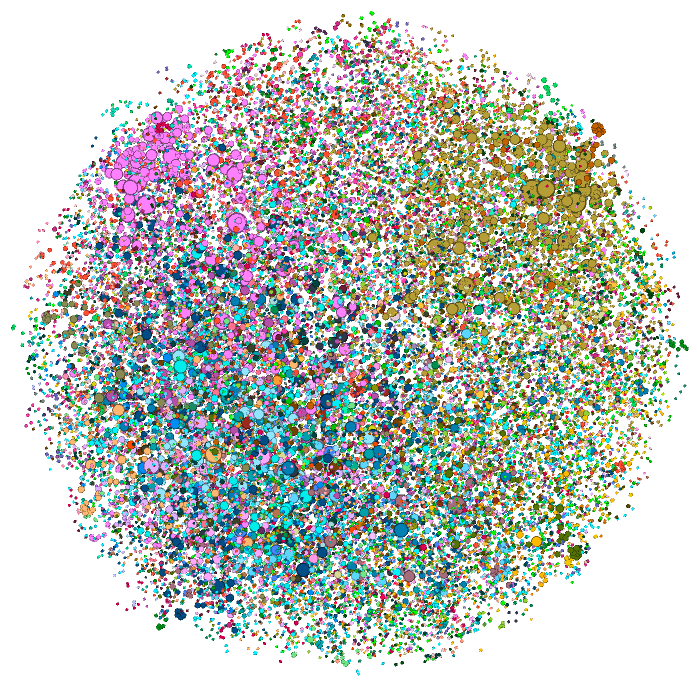
\includegraphics[width=12cm]{img/grafo_overview.png}
\caption{Visão geral das comunidades utilizando partição de modularidade no Gephi}
\label{fig:grafo_overview}
\end{figure}


\section{Rankeamento e centralidade vértices}

Do ponto de vista individual das entidades ou vértices da rede, com frequência é pertinente à aplicação estabelecer algum critério para classificar os vértices mais importantes. Essa importância denotada não é um conceito rígido e final, mas que flexivelmente depende do contexto da aplicação e passível de interpretação. Em cada cenário possível (estratégias de marketing, no estudo de disseminação de doenças, dentre outros exemplos) a escolha de uma métrica ou critério pode tomar uma conotação diferente. Para ilustrar essas possibilidades, 4 métricas são aplicadas para obter os vértices mais bem classificados segundo esses critérios.

O primeiro deles, o grau de entrada refere-se de forma direta ao número de conexões (ou, no contexto da base, quem co-atuou com mais atores diferentes). A centralidade de proximidade (\textit{closeness}) é uma forma de detectar nós que são capazes de espalhar informações de forma eficiente e mede sua distância média para todos os outros nós. A centralidade por intermediação (\textit{betweenness}) refere-se ao número de menores caminhos de todos os vértices para quaisquer outros vértices que passam por aquele nó. Por fim, a centralidade por auto-vetor é baseada na noção de que a influência de um vértice é dada não de forma individual, mas existe uma influência mútua, onde um vértice que faz interação com um vértice de maior influência, é potencialmente um vértice com maior influência (ideia base do algoritmo de \textit{pagerank}). A tabela \ref{tab:rankeamento vertices} apresenta os atores melhor classificados em cada critério, juntamente com o respectivo índice.

\begin{table}[h]
\footnotesize
\centering

\caption{Rankeamento e centralidade dos vértices} % igual ao ambiente figura
\begin{tabular}{|m{3.5cm}|m{3.5cm}|m{3.5cm}| m{3.5cm}|}

\hline
\multicolumn{1}{|c|}{\textbf{Maior Grau}} & \multicolumn{1}{c|}{\textbf{Betweenness}} & \multicolumn{1}{c|}{\textbf{Closeness}} & \multicolumn{1}{c|}{\textbf{Auto-vetor}} \\
\hline


Anupam Kher: 277 & Anupam Kher: 0.059 & Gerard Butler: 0.267
 & Takahiro Sakurai: 0.16\\
\hline

Shah Rukh Khan: 212 & Om Puri: 0.03 & Alfred Molina: 0.265 & Yuichi Nakamura: 0.15\\
\hline

Takahiro Sakurai: 208 & Sahajak Boonthanakit: 0.028 & Ben Kingsley: 0.264 & Yuki Kaji: 0.15\\
\hline

Yuki Kaji: 202 & Iko Uwais: 0.026 & Chloe Grace Moretz: 0.263 & Jun Fukuyama: 0.14\\
\hline

Fred Tatasciore: 197 & Ben Kingsley: 0.025 & Helen Mirren: 0.262 & Junichi Suwabe: 0.13\\
\hline

Yuichi Nakamura: 196 & Cesar Montano: 0.025 & James Franco: 0.262 & Katsuyuki Konishi: 0.13\\
\hline

Fred Armisen: 189 & Steven Yeun: 0.025 & Samuel L. Jackson: 0.261 & Kana Hanazawa: 0.12\\
\hline

Akshay Kumar: 188 & Kari Wahlgren: 0.022 & Jacki Weaver: 0.261 & Eri Kitamura: 0.12 \\
\hline

Om Puri: 187 & Haluk Bilginer: 0.021 & Lena Headey: 0.261 & Daisuke Ono:  0.12\\
\hline

Boman Irani: 183 & Christopher Lee: 0.021 & Willem Dafoe: 0.260 & Hiroshi Kamiya: 0.12\\

\hline
\end{tabular}
\label{tab:rankeamento vertices}
\end{table}



\section{Comparação com o processo de geração aleatório (Erdõs-Rényi)}

Para a etapa de inspeção e verificação com relação ao quanto a formação da rede se aproxima de um processo aleatório, gerou-se um modelo de Erdős–Rényi utilizando os parâmetros da componente principal para quantidade de nós e densidade. A rede obtida, como esperado, tem 29.440 nós e um número bem próximo de arestas (241.853, que anteriomente eram 241.744). O grafo gerado possui um único componente conectado, que por definição é também a componente gigante.

Os coeficientes de aglomeração/triangulação, por sua vez, são significativamente menores que a rede original (o que é esperado, já que não segue a definição do modelo que gera os cliques): 0.000587 e 0.000582, respectivamente. A diferença na formação das redes fica evidente ao observar a distribuição de graus dos nós na figura \ref{fig:comparacao}. Enquanto a rede em estudo segue uma lei de potência em sua distribuição (característica de redes do mundo real), a rede gerada aleatoriamente segue uma distribuição normal (característica de redes geradas aleatoriamente).


\begin{figure}[H]
	\centering
  	\subfigure[Rede em estudo (Netflix)]{
   	 	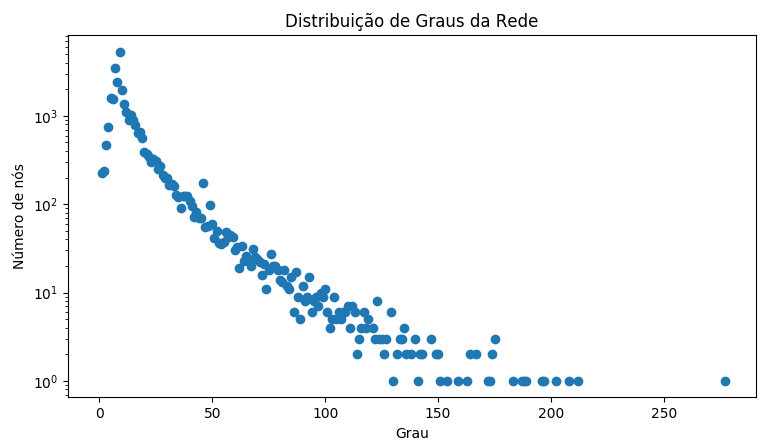
\includegraphics[width=12cm]{img/grau-netflix.png}
    		\label{subfig:grau-netflix}}
    		\hfill
  	\subfigure[Rede de Erdős–Rényi]{
    		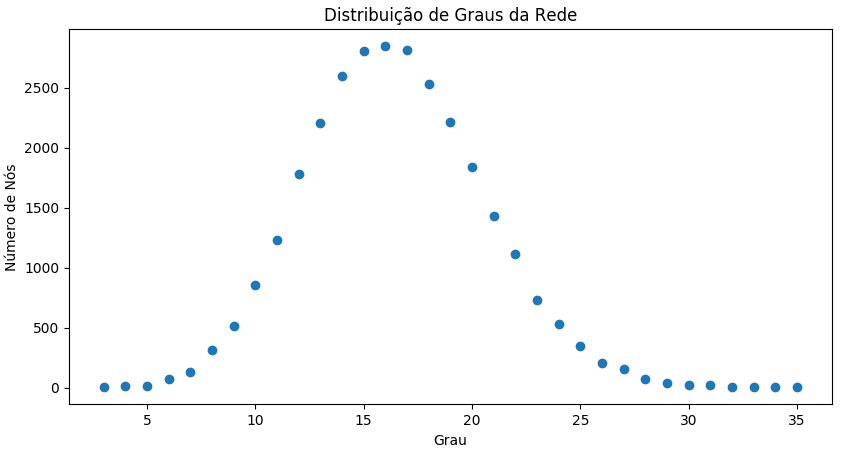
\includegraphics[width=12cm]{img/grau-erdos.png}
    		\label{subfig:grau-erdos}} 
  	\caption{Distribuição de graus}  
  	\label{fig:comparacao}
\end{figure}	
	


% ----------------------------------------------------------
% PARTE - preparação da pesquisa
% ----------------------------------------------------------
%\part{Metodologia} %Preparação da Pesquisa

% Aqui entram os capítulos relacionados à metodologia da pesquisa a ser realizada
\chapter{Predição de sucesso utilizando a nota de avaliação do IMDB}

A hipótese a ser analisada no processo pode ser descrita como: "para cada nó, é possível predizer sua nota com base nas notas dos vizinhos (ou seja, aqueles que atuaram com ele em algum momento)?". Em um teste inicial de viabilidade, verifica-se uma alta correlação entre a nota do ator e a média dos vizinhos utilizando a correlação de Pearson. O cálculo apontou uma correlação de 0,96 entre o conjunto de valores de notas dos vértices e a média das notas dos seus vizinhos imediatos. Essa alta correlação é consequência também da formação dos cliques, já que o vértice possui muitos vizinhos imediatos com uma nota próxima (ainda ponderado pela quantidade de elementos da vizinhança).

Utilizando a média como forma direta de predição, e comparando com a nota efetiva, é possível obter uma estimativa da acurácia. Neste caso, como forma de avaliação, é calculado o erro quadrático entre o valor predito e o real, e para toda a rede, obtém-se o erro médio. Neste caso, o erro médio obtido foi de 0,25 em notas que variam de 0 a 10. Ainda que o erro seja baixo, uma opção de modelo para predição é utilizar os conjuntos de valores para definir uma função linear que possa predizer melhor a nota com base na média. 

\begin{figure}[!htb]
\centering
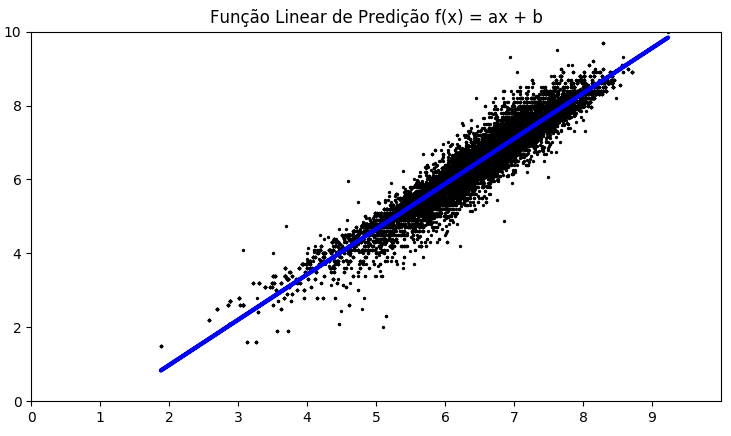
\includegraphics[width=15cm]{img/funcaolinear.png}
\caption{Função linear para melhor aproximação do conjunto de dados}
\label{fig:funcaolinear}
\end{figure}

A figura \ref{fig:funcaolinear} ilustra a dispersão dos valores e a reta que melhor estima os valores. Utilizando regressão linear, a função linear de variável simples que descreve essa reta é dada por f(x) = 1.22x - 1.47. Utilizando essa função para fazer a predição, o erro médio cai para 0,21(...). 
Indo um pouco além, outra hipótese é considerar um modelo multi-variável que considere as médias de vizinhos a distâncias N do vértice. Por exemplo, para N=2, a média dos vizinhos dos vizinhos também são consideradas para tentar ajustar melhor o modelo. Efetuando o primeiro teste para modelo multi-variável com N=2, obteve-se a função f(x) = 1.29x\textsubscript{1} + - 0.26x\textsubscript{2} - 0.19 (onde x\textsubscript{1} é a média dos vizinhos diretos, enquanto x\textsubscript{2} é a média dos vizinhos dos vizinhos). No entando, ao efetuar o teste de predição, o erro médio obtido foi da mesma ordem de 0.21(...), não justificando seu custo computacional.

Utilizando então a função linear obtida para predição, é possível tomar o seguinte cenário hipotético para ilustrar: um ator X, não conhecido previamente, mas que se sabe que atuou com Will Smith, Adam Sandler, Mila Kunis, Keanu Reeves, Rodrigo Santoro e Carrie Fisher (ilustrado na figura \ref{fig:predict}. O valor predito da sua média é obtido substituindo a variável na função pela média desses vizinhos. Esse valor seria dado então por 1,22 * 6,31 - 1,47 = 6,23.


\begin{figure}[!htb]
\centering
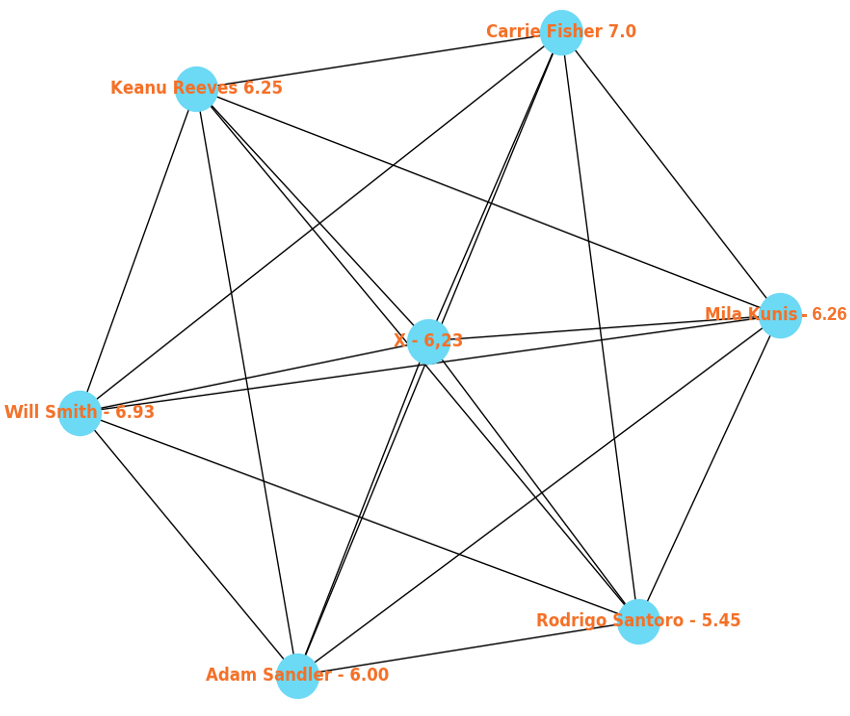
\includegraphics[width=16cm]{img/predict.png}
\caption{Cenário utilizando na predição}
\label{fig:predict}
\end{figure}



% ----------------------------------------------------------
% Resultados
% ----------------------------------------------------------
%\part{Resultados}

%Aqui entram os capitulos contendo a análise e discussão dos resultados. A conclusão fica logo abaixo, em um capítulo sem numeração
% ---	
% primeiro capitulo de Resultados
% ---
%\chapter{Discussão da análise e dos resultados}


% ---
% Finaliza a parte no bookmark do PDF, para que se inicie o bookmark na raiz
% ---
\bookmarksetup{startatroot}% 
% ---

% ---
% Conclusão
% ---
\chapter*[Conclusão]{Conclusão}
\addcontentsline{toc}{chapter}{Conclusão}

O Tim Sort, como algoritmo híbrido, tira vantagem do fato de que, em aplicações no mundo real, frequentemente são encontrados padrões nos quais sub-conjuntos de uma lista já estão ordenados. Se beneficiando dessa característica e fazendo uso das funções de ordenação do Insertion e Merge Sort para uma estratégia de divisão e conquista, o algoritmo se mostra muito eficiente aos cenários em que é submetido na prática e acabou se tornando o método padrão das linguagens Python e Java SE 7.

Para trabalhos futuros, sugerem-se algumas otimizações que visam melhorar ainda mais o desempenho do Tim Sort, como por exemplo a ordenação por inserção com busca binária e o merge com galopeamento binário. A implementação aqui demonstrada na linguagem python, ainda que menos verbosa e de mais fácil compreensão, é menos eficiente do que uma linguagem de mais baixo nível, como C. Essa transcrição também é sugerida como melhoria em termos de performance.

Por fim, o trabalho aqui proposto é também uma demonstração de análise e comparação de diferentes algoritmos para solução de um mesmo problema. A partir da análise teórica de complexidade das rotinas propostas, a verificação prática se dá para confirmar o comportamento assintótico dessas soluções em diferentes contextos à medida que são sobrecarregados com entradas de diversas escalas. Em um caso de uso real, esse processo vem apoiar a tomada de decisão de acordo com o cenário em questão.

% ----------------------------------------------------------
% ELEMENTOS PÓS-TEXTUAIS
% ----------------------------------------------------------
\postextual

% ----------------------------------------------------------
% Referências bibliográficas
% ----------------------------------------------------------

%\bibliography{referencias}

% ----------------------------------------------------------
% Glossário
% ----------------------------------------------------------
%
% Consulte o manual da classe abntex2 para orientações sobre o glossário.
%
%\glossary

% ----------------------------------------------------------
% Apêndices - Caso não existam, comentar
% ----------------------------------------------------------

% ----------------------------------------------------------
% Anexos - Caso não existam, comentar
% ----------------------------------------------------------
%% ---
% Inicia os anexos
% ---
\begin{anexosenv}

% Imprime uma página indicando o início dos anexos
\partanexos

% ---
\chapter{Avaliação de Acessibilidade pelo \textit{Software} Hera}
% ---

\end{anexosenv}


%---------------------------------------------------------------------
% INDICE REMISSIVO
%---------------------------------------------------------------------
\printindex


\begin{thebibliography}{9}



\bibitem{b2}\textbf{Insertion Sort Algorithm}. Disponível em: <\href{https://www.tutorialspoint.com/data\_structures\_algorithms/insertion\_sort\_algorithm.htm}{https://www.tutorialspoint.com/data\_structures\_algorithms/insertion\_sort\_algorithm.htm}>. Acesso em março de 2021.

\bibitem{b2}\textbf{Merge Sort Algorithm}. Disponível em: <\href{https://www.tutorialspoint.com/data\_structures\_algorithms/merge\_sort\_algorithm.htm
}{https://www.tutorialspoint.com/data\_structures\_algorithms/merge\_sort\_algorithm.htm
}>. Acesso em março de 2021.

\bibitem{b2}\textbf{Tim Sort Algorithm}. Disponível em: <\href{https://www.geeksforgeeks.org/timsort/}{https://www.geeksforgeeks.org/timsort/}>. Acesso em março de 2021.

\bibitem{b2}\textbf{An Introduction to Algorithm Complexity Analysis}. Disponível em: <\href{https://discrete.gr/complexity/}{https://discrete.gr/complexity/}>. Acesso em março de 2021.




\end{thebibliography}

\end{document}

